% ══════════════════════════════════════════════════════════════════════════════
% 期中報告（中文）— 內容移植自 document/group_meeting/2026-08-24/report.tex
% 編譯方式：LuaLaTeX，見 .latexmkrc
% ══════════════════════════════════════════════════════════════════════════════
\documentclass[12pt,fontset=none]{ctexart}

% ── Packages ──────────────────────────────────────────────────────────────────
\usepackage[margin=1in]{geometry}
\usepackage{amsmath, amssymb}
\usepackage{graphicx}
\usepackage{booktabs}
\usepackage[hidelinks]{hyperref}
\usepackage{caption}

% ── CJK font: DFKai-SB (標楷體) on Windows, falling back to AR PL KaitiM Big5
% (a metric/style-compatible open Kaiti substitute) when DFKai-SB isn't
% installed (e.g. Linux: apt install fonts-arphic-bkai00mp).
% fontset=none disables ctex's auto-detected Simplified-Chinese fonts
% (SimHei/KaiTi), which aren't installed on this Traditional-Chinese system.
\IfFontExistsTF{DFKai-SB}{%
  \setCJKmainfont{DFKai-SB}
  \setCJKsansfont{DFKai-SB}
  \setCJKmonofont{DFKai-SB}
}{%
  \setCJKmainfont{AR PL KaitiM Big5}
  \setCJKsansfont{AR PL KaitiM Big5}
  \setCJKmonofont{AR PL KaitiM Big5}
}

% ── Traditional-Chinese wording overrides ──────────────────────────────────────
% ctex's built-in auto-generated names (contentsname/figurename/refname)
% default to Simplified Chinese; override them for a Traditional document.
\renewcommand{\contentsname}{目錄}
\renewcommand{\figurename}{圖}
\renewcommand{\refname}{參考文獻}

% ── Metadata ──────────────────────────────────────────────────────────────────
\title{星載合成孔徑雷達船舶偵測之建模與評估\\期中報告}
\author{陳仁澤}
\date{\today}

% plain: no running header (section name), just the page number, centered
% at the bottom -- overrides ctexart's default "headings" style.
\pagestyle{plain}

\begin{document}

% ── Cover page ──────────────────────────────────────────────────────────────
% Custom titlepage (instead of \maketitle) to show the funded project name,
% PI, research assistant, and execution period alongside the report title.
\begin{titlepage}
  \centering
  \vspace*{2cm}
  {\LARGE\bfseries 計畫名稱：基於壓縮感測之合成孔徑雷達即時成像演算法\par}
  \vspace{1.5cm}
  {\Large 星載合成孔徑雷達船舶偵測之建模與評估\par}
  {\Large 期中報告\par}
  \vspace{4cm}
  {\large
    \begin{tabular}{r@{\hspace{0.5em}}l}
      計畫主持人： & 國立台灣大學重點科技學院\ 蔡佩芸 \\[0.6em]
      研究助理：   & 陳仁澤 \\[0.6em]
      執行期間：   & 2026/3 -- 2026/9（期中）\\
    \end{tabular}
  }
  \vfill
\end{titlepage}

\tableofcontents

% ══════════════════════════════════════════════════════════════════════════════
\section{緒論與研究動機}

\subsection{背景}
合成孔徑雷達（SAR）原始資料透過下傳鏈路傳送至地面站，並在地面完成聚焦成像、影像強化與船舶偵測；偵測到的船舶目標可提供海事監控所需的位置與目標資訊。

\begin{figure}[htbp]
  \centering
  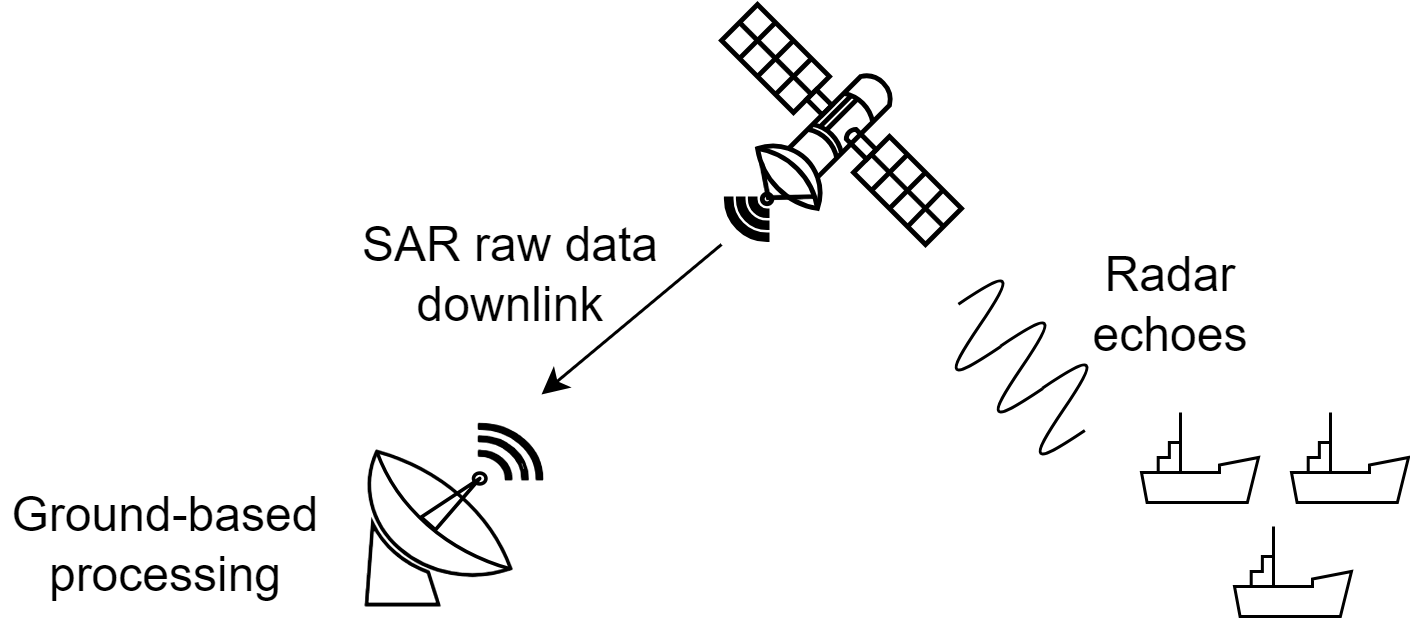
\includegraphics[width=0.6\textwidth]{../../group_meeting/figures/intro/ground_based_sar_ship_detection.png}
  \caption{地面式 SAR 船舶偵測處理流程示意圖。}
\end{figure}

\subsection{問題與動機}
\begin{itemize}
  \item \textbf{地面式處理}：原始資料量大、下傳頻寬有限，導致目標資訊延遲。
  \item \textbf{星載（onboard）處理}：僅需下傳偵測到的目標資訊而非完整原始資料，可降低下傳鏈路頻寬需求，並縮短從下傳到地端處理完成的延遲，但受限於運算能力、記憶體與功耗。
  \item \textbf{研究目標}：發展輕量化的 SAR 處理方法，以達成低延遲的船舶偵測。
\end{itemize}

% ══════════════════════════════════════════════════════════════════════════════
\section{評估架構}

\subsection{整體評估流程}
本研究聚焦於「強化 SAR 成像」，並以 YOLO-based 船舶偵測作為評估任務，整體流程如圖 \ref{fig:eval-framework} 所示：從點散射體回波模型產生原始回波，經過強化 SAR 成像後，再送入 YOLO 偵測模型評估表現。

\begin{figure}[htbp]
  \centering
  
\includegraphics[width=\textwidth]{../../group_meeting/figures/pipeline/evaluation_framework.png}
  \caption{評估架構管線：點散射體回波模型 $\to$ 強化 SAR 成像（研究重點）$\to$ YOLO 船舶偵測 $\to$ 效能評估。}
  \label{fig:eval-framework}
\end{figure}

\subsection{評估指標}
\begin{itemize}
  \item Precision $= \dfrac{TP}{TP+FP}$，Recall $= \dfrac{TP}{TP+FN}$
  \begin{itemize}
    \item[] TP：True Positive；FP：False Positive；FN：False Negative
  \end{itemize}
  \item mAP@0.5：在 IoU 門檻值 0.5 下，跨類別的平均精確度（Mean Average Precision）
  \begin{itemize}
    \item[] IoU（Intersection over Union）＝ 預測框與真實框的重疊面積 / 聯集面積
  \end{itemize}
\end{itemize}

\begin{figure}[htbp]
  \centering
  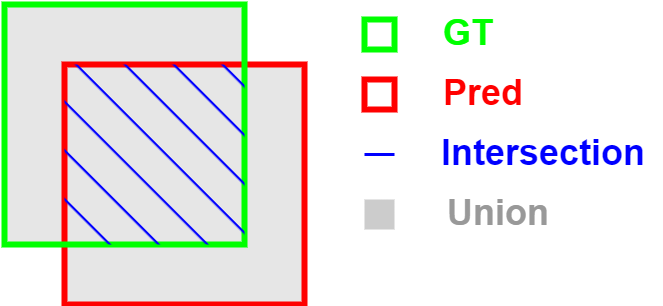
\includegraphics[width=0.35\textwidth]{../../group_meeting/figures/pipeline/iou_def.png}
  \caption{IoU 定義示意圖：GT 為真實標註框，Pred 為預測框，IoU＝交集（Intersection）面積除以聯集（Union）面積。}
\end{figure}
上述指標定義參考自文獻 \cite{sares_deim}。

\subsection{資料集與偵測模型設定}
本研究使用 HRSID（High-Resolution SAR Images Dataset）資料集 \cite{hrsid}：
\begin{itemize}
  \item 訓練集：3,642 張影像；驗證集：1,962 張影像
  \item 影像尺寸：$800 \times 800$ 像素
\end{itemize}
偵測模型採用 YOLO11m，於 HRSID 上微調訓練 100 個 epoch，驗證表現如表 \ref{tab:val-perf}。

\begin{table}[htbp]
  \centering
  \caption{YOLO11m 於 HRSID 驗證集上的表現。}
  \label{tab:val-perf}
  \begin{tabular}{lc}
    \toprule
    指標 & 數值 \\
    \midrule
    Precision & 0.910 \\
    Recall    & 0.840 \\
    mAP@0.5   & 0.922 \\
    \bottomrule
  \end{tabular}
\end{table}

\begin{figure}[htbp]
  \centering
  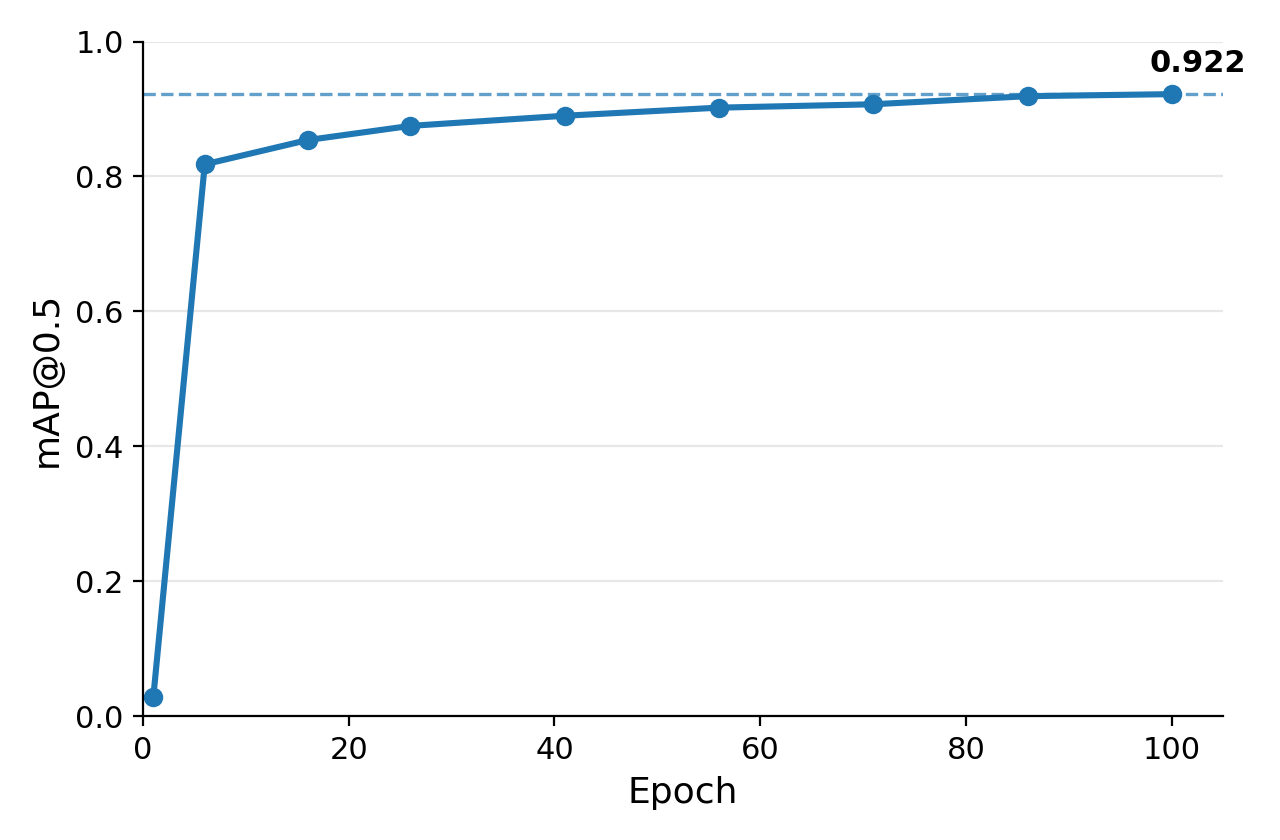
\includegraphics[width=0.6\textwidth]{../../group_meeting/figures/yolo/map_vs_epoch.png}
  \caption{訓練過程中 mAP@0.5 隨 epoch 數的變化。}
\end{figure}

\subsection{YOLO 船舶偵測結果}
在 HRSID 驗證集（1,962 張影像，其中近岸 369 張、離岸 1,593 張）上，依場景分類的偵測結果如表 \ref{tab:yolo-results} 所示；離岸場景的偵測表現優於近岸場景 \cite{balance_scene}。
表 \ref{tab:val-perf} 使用 GPU 進行 inference，表 \ref{tab:yolo-results} 改用 CPU 進行 inference，因此兩表數值略有差異；表 \ref{tab:yolo-results} 之後的所有實驗皆使用 CPU 進行 inference。

\begin{table}[htbp]
  \centering
  \caption{YOLO 船舶偵測結果（依場景分類）。}
  \label{tab:yolo-results}
  \begin{tabular}{lccc}
    \toprule
     & 全體 & 近岸 & 離岸 \\
    \midrule
    影像數    & 1,962 & 369   & 1,593 \\
    Precision & 0.913 & 0.803 & 0.982 \\
    Recall    & 0.846 & 0.741 & 0.965 \\
    mAP@0.5   & 0.918 & 0.817 & 0.984 \\
    \bottomrule
  \end{tabular}
\end{table}

\begin{figure}[htbp]
  \centering
  \begin{minipage}{0.48\textwidth}
    \centering
    
\includegraphics[width=\linewidth]{../../group_meeting/figures/yolo/inshore_example_gt_vs_pred.png}
    \caption*{近岸範例}
  \end{minipage}
  \hfill
  \begin{minipage}{0.48\textwidth}
    \centering
    
\includegraphics[width=\linewidth]{../../group_meeting/figures/yolo/offshore_example_gt_vs_pred.png}
    \caption*{離岸範例}
  \end{minipage}
  \caption{真實標註框（GT）與預測框（Pred）比較範例。}
\end{figure}

% ══════════════════════════════════════════════════════════════════════════════
\section{SAR 回波與成像模型}

\subsection{點散射體回波模型：幾何關係}
輸入 SAR 影像中每個像素的 range location（行）、azimuth location（列）與 intensity（強度值），分別轉換為對應散射體的 range、Doppler（即下述之距離偏移 $d_k$、方位時間偏移 $\Delta\eta_k$）與 magnitude（散射係數 $A_k$，見下節訊號合成）。由於 SAR 系統量測的是斜距，此處假設場景平面高度為零，即斜距（slant range）等於地距（ground range），因此可直接以像素對應的地距偏移作為斜距偏移的近似。

目標位置決定了隨慢時間 $\eta_m$ 變化的斜距 $R_k(\eta_m)$：
\begin{equation}
  R_k(\eta_m) = \sqrt{R_{0,k}^2 + (\eta_m + \Delta\eta_k)^2 V_r^2}
\end{equation}
其中 $R_{0,k} \approx R_0 + d_k$：
\begin{itemize}
  \item $R_0$：場景中心的斜距
  \item $d_k$：散射體 $k$ 相對場景中心的距離偏移（以斜距方向近似）
  \item $\eta_m = m\Delta\eta$：慢時間
  \item $\Delta\eta_k$：散射體 $k$ 相對場景中心的方位時間偏移
\end{itemize}

\begin{figure}[htbp]
  \centering
  
\includegraphics[width=0.55\textwidth]{../../group_meeting/figures/point_scatterer/point_target_geometry.png}
  \caption{點散射體回波模型幾何關係示意圖。}
\end{figure}

\subsection{訊號合成}
延遲與相位皆為幾何相依：
\begin{equation}
  \tau_k(\eta_m) = \frac{2R_k(\eta_m)}{c}, \qquad
  \phi_k(\eta_m) = -4\pi \frac{R_k(\eta_m)}{\lambda}
\end{equation}
回波訊號矩陣 $\mathbf{S} = [s_{m,n}]_{M\times N}$ 由下式合成：
\begin{equation}
  s_{m,n} = \sum_k A_k\,\mathrm{rect}\!\left(\frac{\tau_n - \tau_k(\eta_m)}{T_r}\right)
    \cdot e^{j\pi K_r\left(\tau_n - \tau_k(\eta_m)\right)^2}
    \cdot e^{j\phi_k(\eta_m)}
\end{equation}
其中：
\begin{itemize}
  \item $\eta_m = m\Delta\eta$：慢時間；$\tau_n = n\Delta\tau$：快時間
  \item $A_k$：散射體 $k$ 的散射係數
  \item $K_r = B_r / T_r$：chirp 調頻率；$B_r$：chirp 頻寬（Hz）；$T_r$：脈衝時寬（秒）
\end{itemize}

% ══════════════════════════════════════════════════════════════════════════════
\section{稀疏影像精修}

\subsection{傳統 SAR 成像}
成像目標為由回波 $\mathbf{Y}$ 還原場景反射率 $\mathbf{H}$。傳統成像方法包含：
\begin{itemize}
  \item RDA（Range Doppler Algorithm，距離都卜勒演算法）
  \item CSA（Chirp Scaling Algorithm，chirp scaling 演算法）
  \item BP（Back-Projection，反投影法）
\end{itemize}

\begin{figure}[htbp]
  \centering
  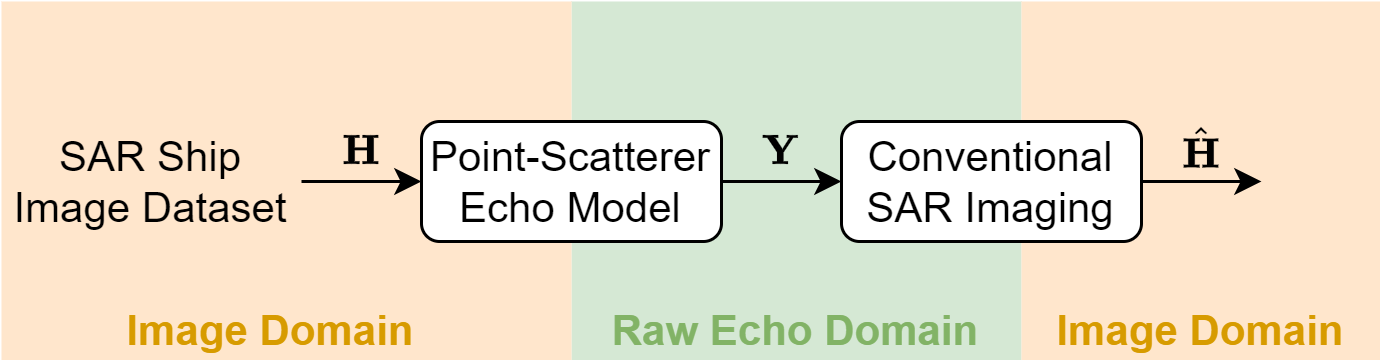
\includegraphics[width=0.5\textwidth]{../../group_meeting/figures/pipeline/sar_imaging_pipeline.png}
  \caption{傳統 SAR 成像管線：點散射體回波模型 $\to$ 傳統 SAR 成像。}
\end{figure}

\subsection{One-Step 稀疏影像精修}
在影像域施加稀疏正則化 \cite{sparse_sar_imaging}：
\begin{equation}
  \hat{\mathbf{H}} = \arg\min_{\mathbf{H}}
    \underbrace{\frac{1}{2}\left\|\mathbf{H}-\mathbf{H}_{\mathrm{CSA}}\right\|_F^2}_{\text{保留 CSA 影像資訊}}
    + \lambda \underbrace{\left\|\mathbf{H}\right\|_1}_{\text{提升稀疏性}}
\end{equation}
此問題可逐元素求得閉式解（soft-thresholding）：
\begin{equation}
  \hat{\mathbf{H}} = \mathcal{S}_\lambda(\mathbf{H}_{\mathrm{CSA}}), \qquad
  \mathcal{S}_\lambda(x) = \frac{x}{|x|}\max(|x|-\lambda, 0),\ x \neq 0
\end{equation}
強散射體被保留，弱散射成分（如背景雜訊）則被抑制，整體處理流程為單一步驟：
\[
  \mathbf{Y} \xrightarrow{\text{CSA}} \mathbf{H}_{\mathrm{CSA}} \xrightarrow{\mathcal{S}_\lambda(\cdot)} \hat{\mathbf{H}}
\]

% ══════════════════════════════════════════════════════════════════════════════
\section{實驗結果}

\subsection{模擬設定}
自 1,593 張離岸 SAR 影像中取樣 100 張作為模擬資料集，於重建後的 SAR 影像上進行船舶偵測評估。SAR 模擬參數如表 \ref{tab:sim-params}。

\begin{table}[htbp]
  \centering
  \caption{SAR 模擬參數。}
  \label{tab:sim-params}
  \begin{tabular}{lclc}
    \toprule
    參數 & 數值 & 參數 & 數值 \\
    \midrule
    脈衝時寬 & 12.5 $\mu$s & 波長 & 0.1152 m \\
    脈衝重複頻率 & 1 kHz & 最近斜距 & 4000 m \\
    頻寬 & 50 MHz & 平台速度 & 120 m/s \\
    取樣頻率 & 64 MHz & 天線長度 & 1.2 m \\
    \bottomrule
  \end{tabular}
\end{table}
目前參數設定採用機載（airborne）平台（如平台速度 120 m/s、最近斜距 4000 m），後續將調整為星載（spaceborne）SAR 系統的典型參數。

\subsection{船舶偵測表現}
精修門檻值設為 120（強度範圍 0–255）。門檻化能抑制 CSA 造成的背景假影，並提升船舶偵測表現，如表 \ref{tab:ship-perf}。
由於本實驗僅自離岸影像中取樣 100 張進行模擬，表 \ref{tab:ship-perf} 中「原始 SAR 影像」的偵測表現與表 \ref{tab:yolo-results}並不完全相同；但由於原始 SAR 影像、CSA、CSA + 稀疏精修三者皆在同一組 100 張影像上評估，彼此之間的比較仍然公平。

\begin{table}[htbp]
  \centering
  \caption{不同處理階段的船舶偵測表現。}
  \label{tab:ship-perf}
  \begin{tabular}{lccc}
    \toprule
    影像 & Precision & Recall & mAP@0.5 \\
    \midrule
    原始 SAR 影像       & 1.000 & 0.978 & 0.975 \\
    CSA                  & 0.977 & 0.940 & 0.954 \\
    CSA + 稀疏精修        & 0.993 & 0.986 & 0.985 \\
    \bottomrule
  \end{tabular}
\end{table}

\subsection{代表性範例}
門檻化能在保留主要船舶響應的同時抑制背景假影，如圖 \ref{fig:representative}。

\begin{figure}[htbp]
  \centering
  \begin{minipage}{0.32\textwidth}
    \centering
    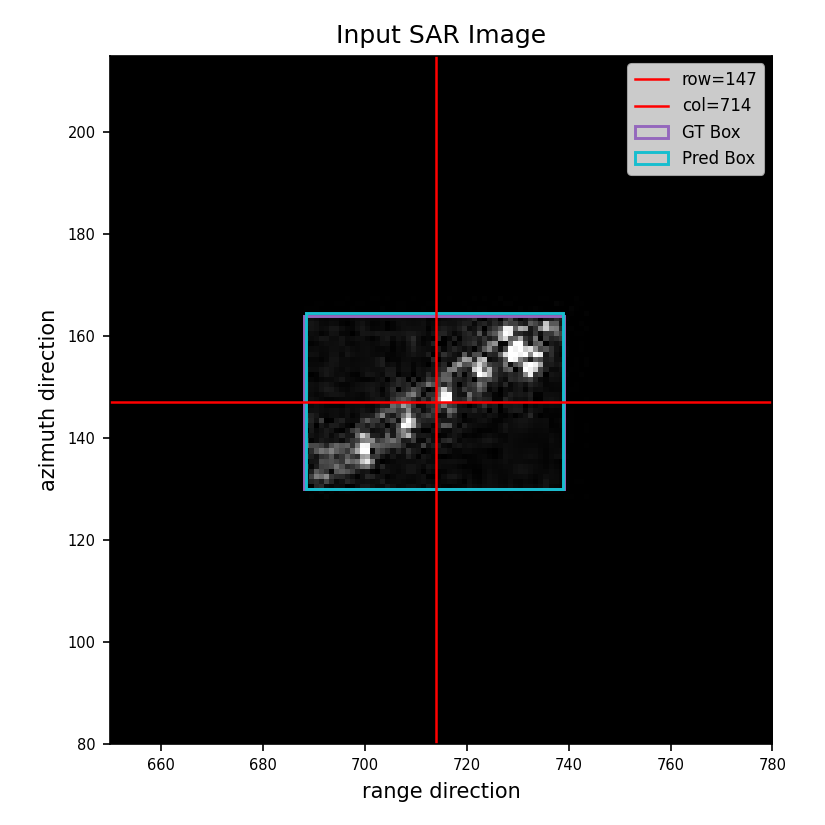
\includegraphics[width=\linewidth]{../../group_meeting/figures/csa_example/input_sar_image.png}
    \caption*{原始輸入}
  \end{minipage}
  \hfill
  \begin{minipage}{0.32\textwidth}
    \centering
    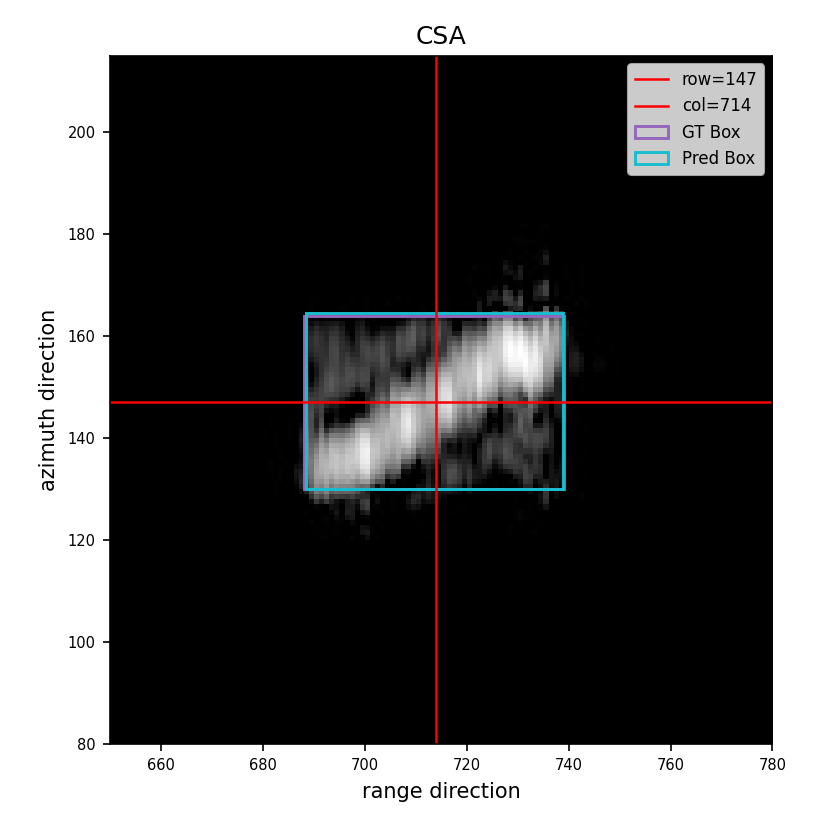
\includegraphics[width=\linewidth]{../../group_meeting/figures/csa_example/csa_output.png}
    \caption*{CSA 輸出}
  \end{minipage}
  \hfill
  \begin{minipage}{0.32\textwidth}
    \centering
    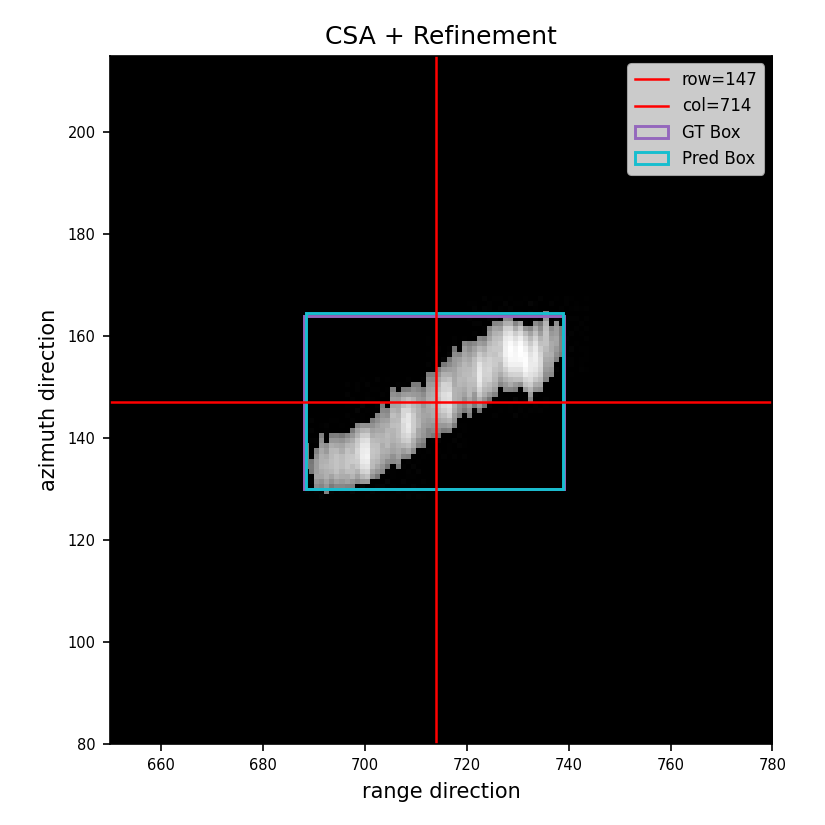
\includegraphics[width=\linewidth]{../../group_meeting/figures/csa_example/csa_threshold_output.png}
    \caption*{CSA + 門檻化}
  \end{minipage}
  \caption{代表性範例比較。}
  \label{fig:representative}
\end{figure}

\subsection{剖面分析}
門檻化能移除低振幅的旁瓣/背景響應，同時保留主要目標結構，如圖 \ref{fig:cross-section} 的距離向與方位向剖面所示。
為了方便比較，圖 \ref{fig:cross-section} 繪製前對強度值做了正規化處理（僅用於繪圖呈現，非 onboard processing 流程的一部分）：soft-thresholding 的結果加回了 $\lambda$（見 4.2 節），且 CSA 與 CSA + 稀疏精修的輸出皆將其峰值正規化至與原始 SAR 影像的峰值一致。

\begin{figure}[htbp]
  \centering
  \begin{minipage}{0.48\textwidth}
    \centering
    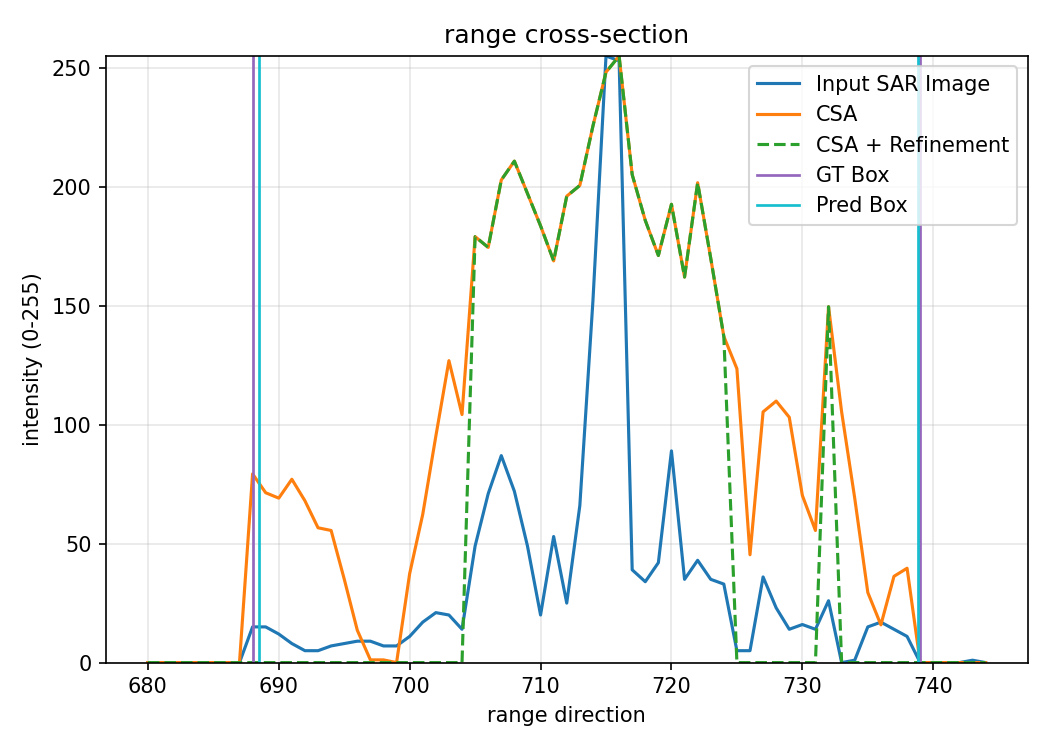
\includegraphics[width=\linewidth]{../../group_meeting/figures/csa_example/range_cross_section.png}
    \caption*{距離向剖面}
  \end{minipage}
  \hfill
  \begin{minipage}{0.48\textwidth}
    \centering
    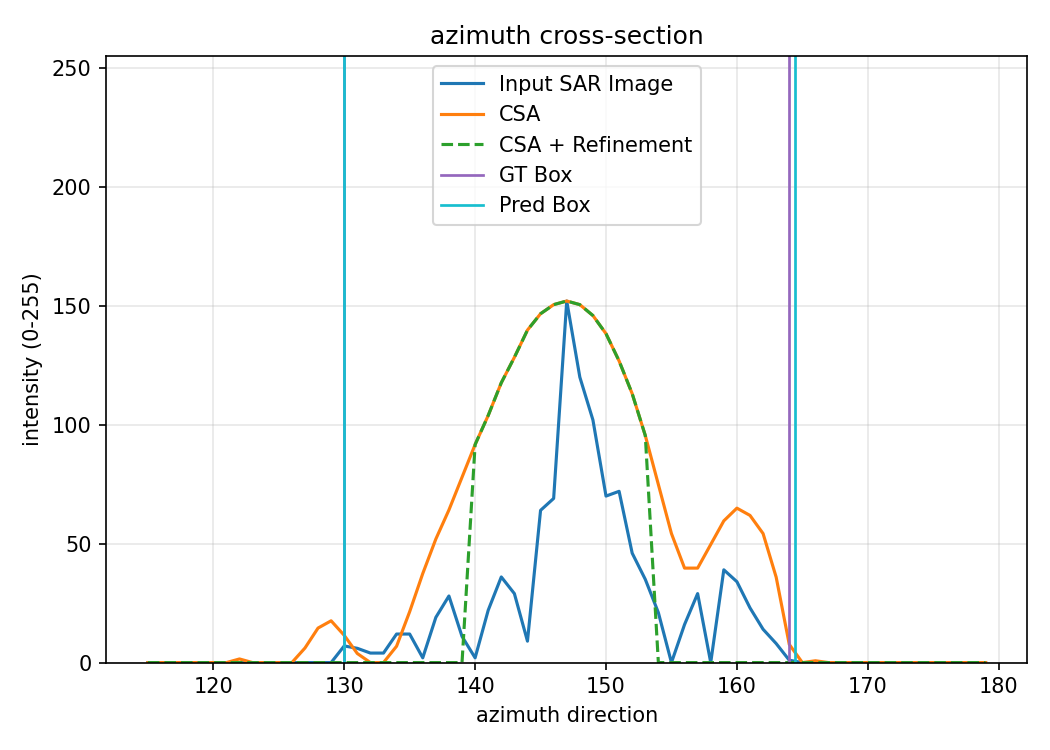
\includegraphics[width=\linewidth]{../../group_meeting/figures/csa_example/azimuth_cross_section.png}
    \caption*{方位向剖面}
  \end{minipage}
  \caption{剖面分析比較。}
  \label{fig:cross-section}
\end{figure}

% ══════════════════════════════════════════════════════════════════════════════
\section{結論}

\subsection{本階段已完成的工作}
\begin{itemize}
  \item 建立了以船舶偵測評估 SAR 影像強化效果的端對端框架。
  \item One-step 稀疏精修能在保留主要船舶響應的同時抑制背景假影。
  \item CSA + 稀疏精修將偵測表現由 mAP@0.5 = 0.954 提升至 0.985。
\end{itemize}

\subsection{後續工作}
\begin{itemize}
  \item 嘗試不同的影像域正則化方法。
  \item 將 speckle noise 納入模擬情境中一併評估。
  \item 將模擬參數由機載（airborne）調整為星載（spaceborne）SAR 系統的典型參數。
\end{itemize}

% ══════════════════════════════════════════════════════════════════════════════
\begin{thebibliography}{9}

\bibitem{sares_deim}
F. Song, S. Yang and X. Zhou, ``SARES-DEIM: Sparse Mixture-of-Experts Meets DETR for Robust SAR Ship Detection,'' in \textit{IEEE Journal of Selected Topics in Applied Earth Observations and Remote Sensing (JSTARS)}, 2026.

\bibitem{hrsid}
S. Wei, X. Zeng, Q. Qu, M. Wang, H. Su and J. Shi, ``HRSID: A High-Resolution SAR Images Dataset for Ship Detection and Instance Segmentation,'' in \textit{IEEE Access}, vol. 8, pp. 120234--120254, 2020.

\bibitem{balance_scene}
T. Zhang \textit{et al.}, ``Balance Scene Learning Mechanism for Offshore and Inshore Ship Detection in SAR Images,'' in \textit{IEEE Geoscience and Remote Sensing Letters}, vol. 19, pp. 1--5, 2022.

\bibitem{sparse_sar_imaging}
H. Bi, G. Bi, B. Zhang, W. Hong and Y. Wu, ``From Theory to Application: Real-Time Sparse SAR Imaging,'' in \textit{IEEE Transactions on Geoscience and Remote Sensing}, vol. 58, no. 4, pp. 2928--2936, April 2020.

\end{thebibliography}

\end{document}
